%%%%%%%%%%%%%%%%%%%%%%%%%%%%%%%%%%%%%%%%%%%%%%%%%
% Chapter: Synchronization and Data Access Operations
%%%%%%%%%%%%%%%%%%%%%%%%%%%%%%%%%%%%%%%%%%%%%%%%%
\chapter{Synchronization and Data Access Operations}
\label{chap:api_sync_acc}

Applications may need to synchronize their operations at various points in
their execution. Depending on a variety of factors (e.g., the programming
model and where the synchronization point lies), the application may choose to
execute the operation using \ac{PMIx}. This is particularly useful in
situations where communication by other means is not yet available since
\ac{PMIx} relies on the host environment's infrastructure for such operations.

Synchronization operations also offer an opportunity for processes to exchange
data at a known point in their execution. Where required, this can include
information on communication endpoints for subsequent wireup of various
messaging protocols.

This chapter covers both the synchronization and data retrieval functions
provided under the \ac{PMIx} Standard.

%%%%%%%%%%%%%%%%%%%%%%%%%%%%%%%%%%%%%%%%%%%%%%%%%
%%%%%%%%%%%%%%%%%%%%%%%%%%%%%%%%%%%%%%%%%%%%%%%%%
\section{\code{PMIx_Fence}}
\declareapi{PMIx_Fence}

%%%%
\summary

Execute a blocking barrier across the processes identified in the specified array, collecting information posted via \refapi{PMIx_Put} as directed.

%%%%
\format

\versionMarker{1.0}
\cspecificstart
\begin{codepar}
pmix_status_t
PMIx_Fence(const pmix_proc_t procs[], size_t nprocs,
           const pmix_info_t info[], size_t ninfo);
\end{codepar}
\cspecificend

\begin{arglist}
\argin{procs}{Array of \refstruct{pmix_proc_t} structures (array of handles)}
\argin{nprocs}{Number of elements in the \refarg{procs} array (integer)}
\argin{info}{Array of info structures (array of handles)}
\argin{ninfo}{Number of elements in the \refarg{info} array (integer)}
\end{arglist}

Returns \refconst{PMIX_SUCCESS} or a negative value corresponding to a PMIx error constant.

\reqattrstart
The following attributes are required to be supported by all \ac{PMIx} libraries:

\pasteAttributeItem{PMIX_COLLECT_DATA}
\pasteAttributeItem{PMIX_COLLECT_GENERATED_JOB_INFO}

\reqattrend

\optattrstart
The following attributes are optional for \ac{PMIx} implementations:

\pasteAttributeItem{PMIX_ALL_CLONES_PARTICIPATE}


The following attributes are optional for host environments:

\pasteAttributeItem{PMIX_TIMEOUT}

\optattrend

%%%%
\descr

Passing a \code{NULL} pointer as the \refarg{procs} parameter indicates that the fence is to span all processes in the client's namespace.
Each provided \refstruct{pmix_proc_t} struct can pass \refconst{PMIX_RANK_WILDCARD} to indicate that all processes in the given namespace are participating.

The \refarg{info} array is used to pass user directives regarding the behavior of the fence operation. Note that for scalability reasons, the default behavior for \refapi{PMIx_Fence} is to not collect data posted by the operation's participants.

\adviceimplstart
\refapi{PMIx_Fence} and its non-blocking form are both \emph{collective} operations. Accordingly, the \ac{PMIx} server library is required to aggregate participation by local clients, passing the request to the host environment once all local participants have executed the \ac{API}.
\adviceimplend

\advicermstart
The host will receive a single call for each collective operation. It is the responsibility of the host to identify the nodes containing participating processes, execute the collective across all participating nodes, and notify the local \ac{PMIx} server library upon completion of the global collective.
\advicermend


%%%%%%%%%%%%%%%%%%%%%%%%%%%%%%%%%%%%%%%%%%%%%%%%%
%%%%%%%%%%%%%%%%%%%%%%%%%%%%%%%%%%%%%%%%%%%%%%%%%
\section{\code{PMIx_Fence_nb}}
\declareapi{PMIx_Fence_nb}

%%%%
\summary

Execute a nonblocking \refapi{PMIx_Fence} across the processes identified in the specified array of processes, collecting information posted via \refapi{PMIx_Put} as directed.

%%%%
\format

\versionMarker{1.0}
\cspecificstart
\begin{codepar}
pmix_status_t
PMIx_Fence_nb(const pmix_proc_t procs[], size_t nprocs,
              const pmix_info_t info[], size_t ninfo,
              pmix_op_cbfunc_t cbfunc, void *cbdata);
\end{codepar}
\cspecificend

\begin{arglist}
\argin{procs}{Array of \refstruct{pmix_proc_t} structures (array of handles)}
\argin{nprocs}{Number of elements in the \refarg{procs} array (integer)}
\argin{info}{Array of info structures (array of handles)}
\argin{ninfo}{Number of elements in the \refarg{info} array (integer)}
\argin{cbfunc}{Callback function (function reference)}
\argin{cbdata}{Data to be passed to the callback function (memory reference)}
\end{arglist}

Returns one of the following:

\begin{itemize}
    \item \refconst{PMIX_SUCCESS}, indicating that the request is being processed by the host environment - result will be returned in the provided \refarg{cbfunc}. Note that the library must not invoke the callback function prior to returning from the \ac{API}.
    \item \refconst{PMIX_OPERATION_SUCCEEDED}, indicating that the request was immediately processed and returned \textit{success} - the \refarg{cbfunc} will \textit{not} be called. This can occur if the collective involved only processes on the local node.
    \item a \ac{PMIx} error constant indicating either an error in the input or that the request was immediately processed and failed - the \refarg{cbfunc} will \textit{not} be called.
\end{itemize}


\reqattrstart
The following attributes are required to be supported by all \ac{PMIx} libraries:

\pasteAttributeItem{PMIX_COLLECT_DATA}
\pasteAttributeItem{PMIX_COLLECT_GENERATED_JOB_INFO}

\reqattrend

\optattrstart
The following attributes are optional for \ac{PMIx} implementations:

\pasteAttributeItem{PMIX_ALL_CLONES_PARTICIPATE}


The following attributes are optional for host environments that support this operation:

\pasteAttributeItem{PMIX_TIMEOUT}

\optattrend

%%%%
\descr

Nonblocking version of the \refapi{PMIx_Fence} routine. See the \refapi{PMIx_Fence} description for further details.

%%%%%%%%%%%%%%%%%%%%%%%%%%%%%%%%%%%%%%%%%%%%%%%%%
\subsection{Fence-related attributes}

The following attributes are defined specifically to support the fence operation:

%
\declareAttribute{PMIX_COLLECT_DATA}{"pmix.collect"}{bool}{
Collect all data posted by the participants using \refapi{PMIx_Put} that
has been committed via \refapi{PMIx_Commit}, making the collection locally
available to each participant at the end of the operation. By default, this will include all job-level information that was locally generated by \ac{PMIx} servers unless excluded using the \refattr{PMIX_COLLECT_GENERATED_JOB_INFO} attribute.
}
%
\declareAttributeProvisional{PMIX_LOCAL_COLLECTIVE_STATUS}{"pmix.loc.col.st"}{pmix_status_t}{
Status code for local collective operation being reported to the host by the server library. PMIx servers may aggregate the participation by local client processes in a collective operation - e.g., instead of passing individual client calls to \refapi{PMIx_Fence} up to the host environment, the server may pass only a single call to the host when all local participants have executed their \refapi{PMIx_Fence} call, thereby reducing the burden placed on the host. However, in cases where the operation locally fails (e.g., if a participating client abnormally terminates prior to calling the operation), the server upcall functions to the host do not include a \refstruct{pmix_status_t} by which the PMIx server can alert the host to that failure. This attribute resolves that problem by allowing the server to pass the status information regarding the local collective operation.
}
\advicermstart
The PMIx server is allowed to pass \refconst{PMIX_SUCCESS} using this attribute, but is not required to do so. PMIx implementations may choose to only report errors in this manner. The lack of an included status shall therefore be taken to indicate that the collective operation locally succeeded.
\advicermend

%
\declareAttributeNEW{PMIX_COLLECT_GENERATED_JOB_INFO}{"pmix.collect.gen"}{bool}{
Collect all job-level information (i.e., reserved keys) that was locally generated by \ac{PMIx} servers. Some job-level information (e.g., distance between processes and fabric devices) is best determined on a distributed basis as it primarily pertains to local processes. Should remote processes need to access the information, it can either be obtained collectively using the \refapi{PMIx_Fence} operation with this directive, or can be retrieved one peer at a time using \refapi{PMIx_Get} without first having performed the job-wide collection.
}
%
\declareAttributeNEW{PMIX_ALL_CLONES_PARTICIPATE}{"pmix.clone.part"}{bool}{
All \refterm{clones} of the calling process must participate in the collective operation.
}


%%%%%%%%%%%%%%%%%%%%%%%%%%%%%%%%%%%%%%%%%%%%%%%%%
%%%%%%%%%%%%%%%%%%%%%%%%%%%%%%%%%%%%%%%%%%%%%%%%%
\section{\code{PMIx_Get}}
\declareapi{PMIx_Get}

%%%%
\summary

Retrieve a key/value pair from the client's namespace.

%%%%
\format

\versionMarker{1.0}
\cspecificstart
\begin{codepar}
pmix_status_t
PMIx_Get(const pmix_proc_t *proc, const pmix_key_t key,
         const pmix_info_t info[], size_t ninfo,
         pmix_value_t **val);
\end{codepar}
\cspecificend

\begin{arglist}
\argin{proc}{Process identifier - a \code{NULL} value may be used in place of the caller's ID (handle)}
\argin{key}{Key to retrieve (\refstruct{pmix_key_t})}
\argin{info}{Array of info structures (array of handles)}
\argin{ninfo}{Number of elements in the \refarg{info} array (integer)}
\argout{val}{value (handle)}
\end{arglist}

Returns one of the following:

\begin{itemize}
\item \refconst{PMIX_SUCCESS} The requested data has been returned in the manner requested (i.e., in a provided static memory location )
\item \refconst{PMIX_ERR_BAD_PARAM} A bad parameter was passed to the function call - e.g., the request included the \refattr{PMIX_GET_STATIC_VALUES} directive, but the provided storage location was \code{NULL}
\item \refconst{PMIX_ERR_EXISTS_OUTSIDE_SCOPE} The requested key exists, but was posted in a \emph{scope} (see Section \ref{api:nres:scope}) that does not include the requester.
\item \refconst{PMIX_ERR_NOT_FOUND} The requested data was not available.
\item a non-zero \ac{PMIx} error constant indicating a reason for the request's failure.
\end{itemize}

\reqattrstart
The following attributes are required to be supported by all \ac{PMIx} libraries:

\pasteAttributeItem{PMIX_OPTIONAL}
\pasteAttributeItem{PMIX_IMMEDIATE}
\pasteAttributeItem{PMIX_DATA_SCOPE}
\pasteAttributeItem{PMIX_SESSION_INFO}
\pasteAttributeItem{PMIX_JOB_INFO}
\pasteAttributeItem{PMIX_APP_INFO}
\pasteAttributeItem{PMIX_NODE_INFO}
\pasteAttributeItem{PMIX_GET_STATIC_VALUES}
\pasteAttributeItem{PMIX_GET_POINTER_VALUES}
\pasteAttributeItem{PMIX_GET_REFRESH_CACHE}

\reqattrend

\optattrstart
The following attributes are optional for host environments:

\pasteAttributeItem{PMIX_TIMEOUT}

\optattrend

%%%%
\descr

Retrieve information for the specified \refarg{key} associated with the process identified in the given \refstruct{pmix_proc_t}. See Chapters \ref{chap:api_rsvd_keys} and \ref{chap:nrkeys} for details on rules governing retrieval of information. Information will be returned according to provided directives:

\begin{itemize}
    \item In the absence of any directive, the returned \refstruct{pmix_value_t} shall be an allocated memory object. The caller is responsible for releasing the object when done.
    \item If \refattr{PMIX_GET_POINTER_VALUES} is given, then the function shall return a pointer to a \refstruct{pmix_value_t} in the \ac{PMIx} library's memory that contains the requested information.
    \item If \refattr{PMIX_GET_STATIC_VALUES} is given, then the function shall return the information in the provided \refstruct{pmix_value_t} pointer. In this case, the caller must provide storage for the structure and pass the pointer to that storage in the \refarg{val} parameter. If the implementation cannot return a static value, then the call to \refapi{PMIx_Get} must return the \refconst{PMIX_ERR_NOT_SUPPORTED} status.
\end{itemize}

This is a blocking operation - the caller will block until the retrieval rules of Chapters \ref{chap:api_rsvd_keys} or \ref{chap:nrkeys} are met.

The \refarg{info} array is used to pass user directives regarding the get operation.

%%%%%%%%%%%%%%%%%%%%%%%%%%%%%%%%%%%%%%%%%%%%%%%%%
\subsection{\code{PMIx_Get_nb}}
\declareapi{PMIx_Get_nb}

%%%%
\summary

Nonblocking \refapi{PMIx_Get} operation.

%%%%
\format

\versionMarker{1.0}
\cspecificstart
\begin{codepar}
pmix_status_t
PMIx_Get_nb(const pmix_proc_t *proc, const char key[],
            const pmix_info_t info[], size_t ninfo,
            pmix_value_cbfunc_t cbfunc, void *cbdata);
\end{codepar}
\cspecificend

\begin{arglist}
\argin{proc}{Process identifier - a \code{NULL} value may be used in place of the caller's ID (handle)}
\argin{key}{Key to retrieve (string)}
\argin{info}{Array of info structures (array of handles)}
\argin{ninfo}{Number of elements in the \refarg{info} array (integer)}
\argin{cbfunc}{Callback function (function reference)}
\argin{cbdata}{Data to be passed to the callback function (memory reference)}
\end{arglist}

Returns one of the following:

\begin{itemize}
    \item \refconst{PMIX_SUCCESS}, indicating that the request is being processed by the host environment - result will be returned in the provided \refarg{cbfunc}. Note that the library must not invoke the callback function prior to returning from the \ac{API}.
    \item a \ac{PMIx} error constant indicating either an error in the input or that the request was immediately processed and failed - the \refarg{cbfunc} will \textit{not} be called.
\end{itemize}

If executed, the status returned in the provided callback function will be one of the following constants:

\begin{itemize}
\item \refconst{PMIX_SUCCESS} The requested data has been returned.
\item \refconst{PMIX_ERR_EXISTS_OUTSIDE_SCOPE} The requested key exists, but was posted in a \emph{scope} (see Section \ref{api:nres:scope}) that does not include the requester.
\item \refconst{PMIX_ERR_NOT_FOUND} The requested data was not available.
\item a non-zero \ac{PMIx} error constant indicating a reason for the request's failure.
\end{itemize}

\reqattrstart
The following attributes are required to be supported by all \ac{PMIx} libraries:

\pasteAttributeItem{PMIX_OPTIONAL}
\pasteAttributeItem{PMIX_IMMEDIATE}
\pasteAttributeItem{PMIX_DATA_SCOPE}
\pasteAttributeItem{PMIX_SESSION_INFO}
\pasteAttributeItem{PMIX_JOB_INFO}
\pasteAttributeItem{PMIX_APP_INFO}
\pasteAttributeItem{PMIX_NODE_INFO}
\pasteAttributeItem{PMIX_GET_POINTER_VALUES}
\pasteAttributeItem{PMIX_GET_REFRESH_CACHE}

\divider

The following attributes are required for host environments that support this operation:

\pasteAttributeItem{PMIX_WAIT}

\reqattrend

\optattrstart
The following attributes are optional for host environments that support this operation:

\pasteAttributeItem{PMIX_TIMEOUT}

\optattrend

%%%%
\descr

The callback function will be executed once the retrieval rules of Chapters \ref{chap:api_rsvd_keys} or \ref{chap:nrkeys} are met.
See \refapi{PMIx_Get} for a full description. Note that the non-blocking form of this function cannot support the \refattr{PMIX_GET_STATIC_VALUES} attribute as the user cannot pass in the required pointer to storage for the result.


%%%%%%%%%%%%%%%%%%%%%%%%%%%%%%%%%%%%%%%%%%%%%%%%%
\subsection{Retrieval attributes}
\label{chap:api_kg:attr}

The following attributes are defined for use by retrieval \acp{API}:

%
\declareAttribute{PMIX_OPTIONAL}{"pmix.optional"}{bool}{
Look only in the client's local data store for the requested value - do not request data from the \ac{PMIx} server if not found.
}
%
\declareAttribute{PMIX_IMMEDIATE}{"pmix.immediate"}{bool}{
Specified operation should immediately return an error from the \ac{PMIx} server if the requested data cannot be found - do not request it from the host \ac{RM}.
}
%
\declareAttributeNEW{PMIX_GET_POINTER_VALUES}{"pmix.get.pntrs"}{bool}{
Request that any pointers in the returned value point directly to values in the key-value store. The user \emph{must not} release any returned data pointers.
}
%
\declareAttributeNEW{PMIX_GET_STATIC_VALUES}{"pmix.get.static"}{bool}{
Request that the data be returned in the provided storage location. The caller is responsible for destructing the \refstruct{pmix_value_t} using the \refmacro{PMIX_VALUE_DESTRUCT} macro when done.
}
%
\declareAttributeNEW{PMIX_GET_REFRESH_CACHE}{"pmix.get.refresh"}{bool}{
When retrieving data for a remote process, refresh the existing local data cache for the process in case new values have been put and committed by the process since the last refresh. Local process information is assumed to be automatically updated upon posting by the process. A \code{NULL} key will cause all values associated with the process to be refreshed - otherwise, only the indicated key will be updated. A process rank of \refconst{PMIX_RANK_WILDCARD} can be used to update job-related information in dynamic environments. The user is responsible for subsequently updating refreshed values they may have cached in their own local memory.
}
%
\declareAttribute{PMIX_DATA_SCOPE}{"pmix.scope"}{pmix_scope_t}{
Scope of the data to be searched in a \refapi{PMIx_Get} call.
}
%
\declareAttribute{PMIX_TIMEOUT}{"pmix.timeout"}{int}{
Time in seconds before the specified operation should time out (zero indicating infinite) and return the \refconst{PMIX_ERR_TIMEOUT} error.
Care should be taken to avoid race conditions caused by multiple layers (client, server, and host) simultaneously timing the operation.
}
%
\declareAttribute{PMIX_WAIT}{"pmix.wait"}{int}{
Caller requests that the \ac{PMIx} server wait until at least the specified number of values are found (a value of zero indicates \emph{all} and is the default).
}


%%%%%%%%%%%%%%%%%%%%%%%%%%%%%%%%%%%%%%%%%%%%%%%%%
%%%%%%%%%%%%%%%%%%%%%%%%%%%%%%%%%%%%%%%%%%%%%%%%%
\section{Query}
\label{chap:api_proc_mgmt:query}

As the level of interaction between applications and the host \ac{SMS} grows, so too does the need for the application to query the \ac{SMS} regarding its capabilities and state information. \ac{PMIx} provides a generalized query interface for this purpose, along with a set of standardized attribute keys to support a range of requests. This includes requests to determine the status of scheduling queues and active allocations, the scope of \ac{API} and attribute support offered by the \ac{SMS}, namespaces of active jobs, location and information about a job's processes, and information regarding available resources.

An example use-case for the \refapi{PMIx_Query_info_nb} \ac{API} is to ensure clean job completion. Time-shared systems frequently impose maximum run times when assigning jobs to resource allocations. To shut down gracefully (e.g., to write a checkpoint before termination) it is necessary for an application to periodically query the resource manager for the time remaining in its allocation. This is especially true on systems for which allocation times may be shortened or lengthened from the original time limit. Many resource managers provide \acp{API} to dynamically obtain this information, but each \ac{API} is specific to the resource manager.

\ac{PMIx} supports this use-case by defining an attribute key (\refattr{PMIX_TIME_REMAINING}) that can be used with the \refapi{PMIx_Query_info_nb} interface to obtain the number of seconds remaining in the current job allocation. Note that one could alternatively use the \refapi{PMIx_Register_event_handler} \ac{API} to register for an event indicating incipient job termination, and then use the \refapi{PMIx_Job_control_nb} \ac{API} to request that the host \ac{SMS} generate an event a specified amount of time prior to reaching the maximum run time. \ac{PMIx} provides such alternate methods as a means of maximizing the probability of a host system supporting at least one method by which the application can obtain the desired service.

The following \acp{API} support query of various session and environment values.


%%%%%%%%%%%%%%%%%%%%%%%%%%%%%%%%%%%%%%%%%%%%%%%%%
\subsection{\code{PMIx_Resolve_peers}}
\declareapi{PMIx_Resolve_peers}

%%%%
\summary

Obtain the array of processes within the specified namespace that are executing on a given node.

%%%%
\format

\versionMarker{1.0}
\cspecificstart
\begin{codepar}
pmix_status_t
PMIx_Resolve_peers(const char *nodename,
                   const pmix_nspace_t nspace,
                   pmix_proc_t **procs, size_t *nprocs);
\end{codepar}
\cspecificend

\begin{arglist}
\argin{nodename}{Name of the node to query - \code{NULL} can be used to denote the current local node (string)}
\argin{nspace}{namespace (string)}
\argout{procs}{Array of process structures (array of handles)}
\argout{nprocs}{Number of elements in the \refarg{procs} array (integer)}
\end{arglist}

Returns \refconst{PMIX_SUCCESS} or a negative value corresponding to a PMIx error constant.

%%%%
\descr

Given a \refarg{nodename}, return the array of processes within the specified \refarg{nspace}
that are executing on that node.
If the \refarg{nspace} is \code{NULL}, then all processes on the node will be returned.
If the specified node does not currently host any processes, then the returned array will be \code{NULL}, and \refarg{nprocs} will be zero.
The caller is responsible for releasing the \refarg{procs} array when done with it.
The \refmacro{PMIX_PROC_FREE} macro is provided for this purpose.


%%%%%%%%%%%%%%%%%%%%%%%%%%%%%%%%%%%%%%%%%%%%%%%%%
\subsection{\code{PMIx_Resolve_nodes}}
\declareapi{PMIx_Resolve_nodes}

%%%%
\summary

Return a list of nodes hosting processes within the given namespace.

%%%%
\format

\versionMarker{1.0}
\cspecificstart
\begin{codepar}
pmix_status_t
PMIx_Resolve_nodes(const char *nspace, char **nodelist);
\end{codepar}
\cspecificend

\begin{arglist}
\argin{nspace}{Namespace (string)}
\argout{nodelist}{Comma-delimited list of nodenames (string)}
\end{arglist}

Returns \refconst{PMIX_SUCCESS} or a negative value corresponding to a PMIx error constant.

%%%%
\descr

Given a \refarg{nspace}, return the list of nodes hosting processes within that namespace.
The returned string will contain a comma-delimited list of nodenames.
The caller is responsible for releasing the string when done with it.


%%%%%%%%%%%%%%%%%%%%%%%%%%%%%%%%%%%%%%%%%%%%%%%%%
\subsection{\code{PMIx_Query_info}}
\declareapi{PMIx_Query_info}

%%%%
\summary

Query information about the system in general.

%%%%
\format

\versionMarker{4.0}
\cspecificstart
\begin{codepar}
pmix_status_t
PMIx_Query_info(pmix_query_t queries[], size_t nqueries,
                pmix_info_t *info[], size_t *ninfo);
\end{codepar}
\cspecificend

\begin{arglist}
\argin{queries}{Array of query structures (array of handles)}
\argin{nqueries}{Number of elements in the \refarg{queries} array (integer)}
\arginout{info}{Address where a pointer to an array of \refstruct{pmix_info_t} containing the results of the query can be returned (memory reference)}
\arginout{ninfo}{Address where the number of elements in \refarg{info} can be returned (handle)}
\end{arglist}

Returns one of the following:

\begin{itemize}
\item \refconst{PMIX_SUCCESS} All data was found and has been returned.

\item \refconst{PMIX_ERR_NOT_FOUND} None of the requested data was available.
The \refarg{info} array will be \code{NULL} and \refarg{ninfo} zero.
\item \refconst{PMIX_ERR_PARTIAL_SUCCESS} Some of the requested data was found.
The \refarg{info} array shall contain an element for each query key that returned a value.

\item \refconst{PMIX_ERR_NOT_SUPPORTED} The host \ac{RM} does not support this function. The \refarg{info} array will be \code{NULL} and \refarg{ninfo} zero.

\item a non-zero \ac{PMIx} error constant indicating a reason for the request's failure. The \refarg{info} array will be \code{NULL} and \refarg{ninfo} zero.
\end{itemize}

\reqattrstart
\ac{PMIx} libraries and host environments that support this \ac{API} are required to support the following attributes:

\pasteAttributeItem{PMIX_QUERY_REFRESH_CACHE}
\pasteAttributeItem{PMIX_SESSION_INFO}
\pasteAttributeItem{PMIX_JOB_INFO}
\pasteAttributeItem{PMIX_APP_INFO}
\pasteAttributeItem{PMIX_NODE_INFO}
\pasteAttributeItem{PMIX_PROC_INFO}
\pasteAttributeItemBegin{PMIX_PROCID}In this context, specifies the process ID whose information is being requested - e.g., a query asking for the \refstruct{pmix_proc_info_t} of a specified process. Only required when the request is for information on a specific process.
\pasteAttributeItemEnd
\pasteAttributeItemBegin{PMIX_NSPACE}Specifies the namespace of the process whose information is being requested. Must be accompanied by the \refattr{PMIX_RANK} attribute. Only required when the request is for information on a specific process.
\pasteAttributeItemEnd
\pasteAttributeItemBegin{PMIX_RANK}Specifies the rank of the process whose information is being requested. Must be accompanied by the \refattr{PMIX_NSPACE} attribute. Only required when the request is for information on a specific process.
\pasteAttributeItemEnd
\pasteAttributeItem{PMIX_QUERY_ATTRIBUTE_SUPPORT}
\pasteAttributeItem{PMIX_CLIENT_ATTRIBUTES}
\pasteAttributeItem{PMIX_SERVER_ATTRIBUTES}
\pasteAttributeItem{PMIX_HOST_ATTRIBUTES}
\pasteAttributeItem{PMIX_TOOL_ATTRIBUTES}

Note that inclusion of both the \refattr{PMIX_PROCID} directive and either the \refattr{PMIX_NSPACE} or the \refattr{PMIX_RANK} attribute will return a \refconst{PMIX_ERR_BAD_PARAM} result, and that the inclusion of a process identifier must apply to all keys in that \refstruct{pmix_query_t}. Queries for information on multiple specific processes therefore requires submitting multiple \refstruct{pmix_query_t} structures, each referencing one process.

\ac{PMIx} libraries are not required to directly support any other attributes for this function. However, all provided attributes must be passed to the host \ac{SMS} daemon for processing. The \ac{PMIx} library is \textit{required} to add the \refAttributeItem{PMIX_USERID} and the \refAttributeItem{PMIX_GRPID} attributes of the client process making the request.

\reqattrend


\optattrstart
The following attributes are optional for host environments that support this operation:

\pasteAttributeItem{PMIX_QUERY_NAMESPACES}
\pasteAttributeItem{PMIX_QUERY_JOB_STATUS}
\pasteAttributeItem{PMIX_QUERY_QUEUE_LIST}
\pasteAttributeItem{PMIX_QUERY_QUEUE_STATUS}
\pasteAttributeItem{PMIX_QUERY_PROC_TABLE}
\pasteAttributeItem{PMIX_QUERY_LOCAL_PROC_TABLE}
\pasteAttributeItem{PMIX_QUERY_SPAWN_SUPPORT}
\pasteAttributeItem{PMIX_QUERY_DEBUG_SUPPORT}
\pasteAttributeItem{PMIX_QUERY_MEMORY_USAGE}
\pasteAttributeItem{PMIX_QUERY_REPORT_AVG}
\pasteAttributeItem{PMIX_QUERY_REPORT_MINMAX}
\pasteAttributeItem{PMIX_QUERY_ALLOC_STATUS}
\pasteAttributeItem{PMIX_TIME_REMAINING}
\pasteAttributeItemBegin{PMIX_SERVER_URI} Requests the URI of the specified \ac{PMIx} server's \ac{PMIx} connection. Defaults to requesting the information for the local \ac{PMIx} server.
\pasteAttributeItemEnd
\pasteAttributeItem{PMIX_CLIENT_AVG_MEMORY}
\pasteAttributeItem{PMIX_DAEMON_MEMORY}
\pasteAttributeItem{PMIX_QUERY_AUTHORIZATIONS}
\pasteAttributeItem{PMIX_PROC_PID}
\pasteAttributeItem{PMIX_PROC_STATE_STATUS}

\optattrend

%%%%
\descr

Query information about the system in general.
This can include a list of active namespaces, fabric topology, etc.
Also can be used to query node-specific info such as the list of peers executing on a given node. The host environment is responsible for exercising appropriate access control on the information.

The returned \refarg{status} indicates if requested data was found or not. The returned \refarg{info} array will contain a \refattr{PMIX_QUERY_RESULTS} element for each query of the \refarg{queries} array. If qualifiers were included in the query, then the first element of each results array shall contain the \refattr{PMIX_QUERY_QUALIFIERS} key with a \refstruct{pmix_data_array_t} containing the qualifiers. The remaining \refstruct{pmix_info_t} shall contain the results of the query, one entry for each key that was found. Note that duplicate keys in the \refarg{queries} array shall result in duplicate responses within the constraints of the accompanying qualifiers. The caller is responsible for releasing the returned array.

\adviceimplstart
Information returned from \refapi{PMIx_Query_info} shall be locally cached so that retrieval by subsequent calls to \refapi{PMIx_Get}, \refapi{PMIx_Query_info}, or \refapi{PMIx_Query_info_nb} can succeed with minimal overhead. The local cache shall be checked prior to querying the \ac{PMIx} server and/or the host environment. Queries that include the \refattr{PMIX_QUERY_REFRESH_CACHE} attribute shall bypass the local cache and retrieve a new value for the query, refreshing the values in the cache upon return.
\adviceimplend


%%%%%%%%%%%%%%%%%%%%%%%%%%%%%%%%%%%%%%%%%%%%%%%%%
\subsection{\code{PMIx_Query_info_nb}}
\declareapi{PMIx_Query_info_nb}

%%%%
\summary

Query information about the system in general.

%%%%
\format

\versionMarker{2.0}
\cspecificstart
\begin{codepar}
pmix_status_t
PMIx_Query_info_nb(pmix_query_t queries[], size_t nqueries,
                   pmix_info_cbfunc_t cbfunc, void *cbdata);
\end{codepar}
\cspecificend

\begin{arglist}
\argin{queries}{Array of query structures (array of handles)}
\argin{nqueries}{Number of elements in the \refarg{queries} array (integer)}
\argin{cbfunc}{Callback function \refapi{pmix_info_cbfunc_t} (function reference)}
\argin{cbdata}{Data to be passed to the callback function (memory reference)}
\end{arglist}

Returns one of the following:

\begin{itemize}
\item \refconst{PMIX_SUCCESS} indicating that the request has been accepted for processing and the provided callback function will be executed upon completion of the operation. Note that the library must not invoke the callback function prior to returning from the \ac{API}.
\item a non-zero \ac{PMIx} error constant indicating a reason for the request to have been rejected. In this case, the provided callback function will not be executed.
\end{itemize}

If executed, the status returned in the provided callback function will be one of the following constants:

\begin{itemize}
\item \refconst{PMIX_SUCCESS} All data was found and has been returned.

\item \refconst{PMIX_ERR_NOT_FOUND} None of the requested data was available.
The \refarg{info} array will be \code{NULL} and \refarg{ninfo} zero.

\item \refconst{PMIX_ERR_PARTIAL_SUCCESS} Some of the requested data was found.
The \refarg{info} array shall contain an element for each query key that returned a value.

\item \refconst{PMIX_ERR_NOT_SUPPORTED} The host \ac{RM} does not support this function. The \refarg{info} array will be \code{NULL} and \refarg{ninfo} zero.

\item a non-zero \ac{PMIx} error constant indicating a reason for the request's failure. The \refarg{info} array will be \code{NULL} and \refarg{ninfo} zero.
\end{itemize}

\reqattrstart
\ac{PMIx} libraries and host environments that support this \ac{API} are required to support the following attributes:

\pasteAttributeItem{PMIX_QUERY_REFRESH_CACHE}
\pasteAttributeItem{PMIX_SESSION_INFO}
\pasteAttributeItem{PMIX_JOB_INFO}
\pasteAttributeItem{PMIX_APP_INFO}
\pasteAttributeItem{PMIX_NODE_INFO}
\pasteAttributeItem{PMIX_PROC_INFO}
\pasteAttributeItemBegin{PMIX_PROCID}In this context, specifies the process ID whose information is being requested - e.g., a query asking for the \refstruct{pmix_proc_info_t} of a specified process. Only required when the request is for information on a specific process.
\pasteAttributeItemEnd
\pasteAttributeItemBegin{PMIX_NSPACE}Specifies the namespace of the process whose information is being requested. Must be accompanied by the \refattr{PMIX_RANK} attribute. Only required when the request is for information on a specific process.
\pasteAttributeItemEnd
\pasteAttributeItemBegin{PMIX_RANK}Specifies the rank of the process whose information is being requested. Must be accompanied by the \refattr{PMIX_NSPACE} attribute. Only required when the request is for information on a specific process.
\pasteAttributeItemEnd
\pasteAttributeItem{PMIX_QUERY_ATTRIBUTE_SUPPORT}
\pasteAttributeItem{PMIX_CLIENT_ATTRIBUTES}
\pasteAttributeItem{PMIX_SERVER_ATTRIBUTES}
\pasteAttributeItem{PMIX_HOST_ATTRIBUTES}
\pasteAttributeItem{PMIX_TOOL_ATTRIBUTES}

Note that inclusion of both the \refattr{PMIX_PROCID} directive and either the \refattr{PMIX_NSPACE} or the \refattr{PMIX_RANK} attribute will return a \refconst{PMIX_ERR_BAD_PARAM} result, and that the inclusion of a process identifier must apply to all keys in that \refstruct{pmix_query_t}. Queries for information on multiple specific processes therefore requires submitting multiple \refstruct{pmix_query_t} structures, each referencing one process.

\ac{PMIx} libraries are not required to directly support any other attributes for this function. However, all provided attributes must be passed to the host \ac{SMS} daemon for processing. The \ac{PMIx} library is \textit{required} to add the \refAttributeItem{PMIX_USERID} and the \refAttributeItem{PMIX_GRPID} attributes of the client process making the request.

\reqattrend

\optattrstart
The following attributes are optional for host environments that support this operation:

\pasteAttributeItem{PMIX_QUERY_NAMESPACES}
\pasteAttributeItem{PMIX_QUERY_JOB_STATUS}
\pasteAttributeItem{PMIX_QUERY_QUEUE_LIST}
\pasteAttributeItem{PMIX_QUERY_QUEUE_STATUS}
\pasteAttributeItem{PMIX_QUERY_PROC_TABLE}
\pasteAttributeItem{PMIX_QUERY_LOCAL_PROC_TABLE}
\pasteAttributeItem{PMIX_QUERY_SPAWN_SUPPORT}
\pasteAttributeItem{PMIX_QUERY_DEBUG_SUPPORT}
\pasteAttributeItem{PMIX_QUERY_MEMORY_USAGE}
\pasteAttributeItem{PMIX_QUERY_REPORT_AVG}
\pasteAttributeItem{PMIX_QUERY_REPORT_MINMAX}
\pasteAttributeItem{PMIX_QUERY_ALLOC_STATUS}
\pasteAttributeItem{PMIX_TIME_REMAINING}
\pasteAttributeItemBegin{PMIX_SERVER_URI} Requests the URI of the specified \ac{PMIx} server's \ac{PMIx} connection. Defaults to requesting the information for the local \ac{PMIx} server.
\pasteAttributeItemEnd
\pasteAttributeItem{PMIX_CLIENT_AVG_MEMORY}
\pasteAttributeItem{PMIX_DAEMON_MEMORY}
\pasteAttributeItem{PMIX_QUERY_AUTHORIZATIONS}
\pasteAttributeItem{PMIX_PROC_PID}
\pasteAttributeItem{PMIX_PROC_STATE_STATUS}

\optattrend

%%%%
\descr

Non-blocking form of the \refapi{PMIx_Query_info} \ac{API}.


%%%%%%%%%%%%%%%%%%%%%%%%%%%%%%%%%%%%%%%%%%%%%%%%%
\subsection{Query-specific constants}
\label{api:struct:constants:query}

\begin{constantdesc}
%
\declareconstitem{PMIX_QUERY_PARTIAL_SUCCESS}
Some, but not all, of the requested information was returned.
%
\end{constantdesc}


%%%%%%%%%%%%%%%%%%%%%%%%%%%%%%%%%%%%%%%%%%%%%%%%%
\subsection{Query attributes}
\label{api:struct:attributes:query}

Attributes used to direct behavior of the \refapi{PMIx_Query_info} \acp{API}.

%
\declareAttributeNEW{PMIX_QUERY_RESULTS}{"pmix.qry.res"}{pmix_data_array_t}{
Contains an array of query results for a given \refstruct{pmix_query_t} passed to the \refapi{PMIx_Query_info} \acp{API}. If qualifiers were included in the query, then the first element of the array shall be the \refattr{PMIX_QUERY_QUALIFIERS} attribute containing those qualifiers. Each of the remaining elements of the array is a \refstruct{pmix_info_t} containing the query key and the corresponding value returned by the query. This attribute is solely for reporting purposes and cannot be used in \refapi{PMIx_Get} or other query operations.
}
%
\declareAttributeNEW{PMIX_QUERY_QUALIFIERS}{"pmix.qry.quals"}{pmix_data_array_t}{
Contains an array of qualifiers that were included in the query that produced the provided results. This attribute is solely for reporting purposes and cannot be used in \refapi{PMIx_Get} or other query operations.
}
%
\declareAttributeNEW{PMIX_QUERY_SUPPORTED_KEYS}{"pmix.qry.keys"}{char*}{
Returns comma-delimited list of keys supported by the query function. NO QUALIFIERS.
}
%
\declareAttributeNEW{PMIX_QUERY_SUPPORTED_QUALIFIERS}{"pmix.qry.quals"}{char*}{
Return comma-delimited list of qualifiers supported by a query on the provided key, instead of actually performing the query on the key. NO QUALIFIERS.
}
%
\declareAttribute{PMIX_QUERY_REFRESH_CACHE}{"pmix.qry.rfsh"}{bool}{
Retrieve updated information from server. NO QUALIFIERS.
}
%
\declareAttribute{PMIX_QUERY_NAMESPACES}{"pmix.qry.ns"}{char*}{
Request a comma-delimited list of active namespaces. NO QUALIFIERS.
}
%
\declareAttributeNEW{PMIX_QUERY_NAMESPACE_INFO}{"pmix.qry.nsinfo"}{pmix_data_array_t*}{
Return an array of active namespace information - each element will itself contain an array including the namespace plus the command line of the application executing within it. OPTIONAL QUALIFIERS: \refattr{PMIX_NSPACE} of specific namespace whose info is being requested.
}
%
\declareAttribute{PMIX_QUERY_JOB_STATUS}{"pmix.qry.jst"}{pmix_status_t}{
Status of a specified, currently executing job. REQUIRED QUALIFIER: \refattr{PMIX_NSPACE} indicating the namespace whose status is being queried.
}
%
\declareAttribute{PMIX_QUERY_QUEUE_LIST}{"pmix.qry.qlst"}{char*}{
Request a comma-delimited list of scheduler queues. NO QUALIFIERS.
}
%
\declareAttribute{PMIX_QUERY_QUEUE_STATUS}{"pmix.qry.qst"}{char*}{
Returns status of a specified scheduler queue, expressed as a string. OPTIONAL QUALIFIERS: \refattr{PMIX_ALLOC_QUEUE} naming specific queue whose status is being requested.
}
%
\pasteAttributeItem{PMIX_QUERY_PROC_TABLE}
%
\pasteAttributeItem{PMIX_QUERY_LOCAL_PROC_TABLE}
%
\declareAttribute{PMIX_QUERY_AUTHORIZATIONS}{"pmix.qry.auths"}{bool}{
Return operations the \ac{PMIx} tool is authorized to perform.  NO QUALIFIERS.
}
%
\declareAttribute{PMIX_QUERY_SPAWN_SUPPORT}{"pmix.qry.spawn"}{bool}{
Return a comma-delimited list of supported spawn attributes. NO QUALIFIERS.
}
%
\declareAttribute{PMIX_QUERY_DEBUG_SUPPORT}{"pmix.qry.debug"}{bool}{
Return a comma-delimited list of supported debug attributes. NO QUALIFIERS.
}
%
\declareAttribute{PMIX_QUERY_MEMORY_USAGE}{"pmix.qry.mem"}{bool}{
Return information on memory usage for the processes indicated in the qualifiers. OPTIONAL QUALIFIERS: \refattr{PMIX_NSPACE} and \refattr{PMIX_RANK}, or \refattr{PMIX_PROCID} of specific process(es) whose memory usage is being requested.
}
%
\declareAttribute{PMIX_QUERY_LOCAL_ONLY}{"pmix.qry.local"}{bool}{
Constrain the query to local information only. NO QUALIFIERS.
}
%
\declareAttribute{PMIX_QUERY_REPORT_AVG}{"pmix.qry.avg"}{bool}{
Report only average values for sampled information. NO QUALIFIERS.
}
%
\declareAttribute{PMIX_QUERY_REPORT_MINMAX}{"pmix.qry.minmax"}{bool}{
Report minimum and maximum values. NO QUALIFIERS.
}
%
\declareAttribute{PMIX_QUERY_ALLOC_STATUS}{"pmix.query.alloc"}{char*}{
String identifier of the allocation whose status is being requested. NO QUALIFIERS.
}
%
\declareAttribute{PMIX_TIME_REMAINING}{"pmix.time.remaining"}{char*}{
Query number of seconds (\code{uint32_t}) remaining in allocation for the specified namespace. OPTIONAL QUALIFIERS: \refattr{PMIX_NSPACE} of the namespace whose info is being requested (defaults to allocation containing the caller).
}
%
\declareAttributeNEW{PMIX_QUERY_ATTRIBUTE_SUPPORT}{"pmix.qry.attrs"}{bool}{
Query list of supported attributes for specified \acp{API}. REQUIRED QUALIFIERS: one or more of \refattr{PMIX_CLIENT_FUNCTIONS}, \refattr{PMIX_SERVER_FUNCTIONS}, \refattr{PMIX_TOOL_FUNCTIONS}, and \refattr{PMIX_HOST_FUNCTIONS}.
}
%
\pasteAttributeItem{PMIX_QUERY_NUM_PSETS}
%
\pasteAttributeItem{PMIX_QUERY_PSET_NAMES}
%
\pasteAttributeItem{PMIX_QUERY_PSET_MEMBERSHIP}
%
\declareAttributeNEW{PMIX_QUERY_AVAIL_SERVERS}{"pmix.qry.asrvrs"}{pmix_data_array_t*}{
Return an array of \refstruct{pmix_info_t}, each element itself containing a \refattr{PMIX_SERVER_INFO_ARRAY} entry holding all available data for a server on this node to which the caller might be able to connect.
}
%
\declareAttributeNEW{PMIX_SERVER_INFO_ARRAY}{"pmix.srv.arr"}{pmix_data_array_t}{
Array of \refstruct{pmix_info_t} about a given server, starting with its \refattr{PMIX_NSPACE} and including at least one of the rendezvous-required pieces of information.
}

\vspace{\baselineskip}
These attributes are used to query memory available and used in the system.

%
\pasteAttributeItemBegin{PMIX_AVAIL_PHYS_MEMORY}OPTIONAL QUALIFERS: \refattr{PMIX_HOSTNAME} or \refattr{PMIX_NODEID} (defaults to caller's node).
\pasteAttributeItemEnd
%
\declareAttribute{PMIX_DAEMON_MEMORY}{"pmix.dmn.mem"}{float}{
Megabytes of memory currently used by the \ac{RM} daemon on the node. OPTIONAL QUALIFERS: \refattr{PMIX_HOSTNAME} or \refattr{PMIX_NODEID} (defaults to caller's node).
}
%
\declareAttribute{PMIX_CLIENT_AVG_MEMORY}{"pmix.cl.mem.avg"}{float}{
Average Megabytes of memory used by client processes on node. OPTIONAL QUALIFERS: \refattr{PMIX_HOSTNAME} or \refattr{PMIX_NODEID} (defaults to caller's node).
}

\vspace{\baselineskip}
The following attributes are used as qualifiers in queries regarding attribute support within the \ac{PMIx} implementation and/or the host environment:

\declareAttributeNEW{PMIX_CLIENT_FUNCTIONS}{"pmix.client.fns"}{bool}{
Request a list of functions supported by the \ac{PMIx} client library.
}
%
\declareAttributeNEW{PMIX_CLIENT_ATTRIBUTES}{"pmix.client.attrs"}{bool}{
Request attributes supported by the \ac{PMIx} client library.
}
%
\declareAttributeNEW{PMIX_SERVER_FUNCTIONS}{"pmix.srvr.fns"}{bool}{
Request a list of functions supported by the \ac{PMIx} server library.
}
%
\declareAttributeNEW{PMIX_SERVER_ATTRIBUTES}{"pmix.srvr.attrs"}{bool}{
Request attributes supported by the \ac{PMIx} server library.
}
%
\declareAttributeNEW{PMIX_HOST_FUNCTIONS}{"pmix.srvr.fns"}{bool}{
Request a list of functions supported by the host environment.
}
%
\declareAttributeNEW{PMIX_HOST_ATTRIBUTES}{"pmix.host.attrs"}{bool}{
Request attributes supported by the host environment.
}
%
\declareAttributeNEW{PMIX_TOOL_FUNCTIONS}{"pmix.tool.fns"}{bool}{
Request a list of functions supported by the \ac{PMIx} tool library.
}
%
\declareAttributeNEW{PMIX_TOOL_ATTRIBUTES}{"pmix.setup.env"}{bool}{
Request attributes supported by the \ac{PMIx} tool library functions.
}


%%%%%%%%%%%%%%%%%%%%%%%%%%%%%%%%%%%%%%%%%%%%%%%%%
\subsection{Query Structure}
\declarestruct{pmix_query_t}

The \refstruct{pmix_query_t} structure is used by the \refapi{PMIx_Query_info} \acp{API} to describe a single query operation.

\versionMarker{2.0}
\cspecificstart
\begin{codepar}
typedef struct pmix_query \{
    char **keys;
    pmix_info_t *qualifiers;
    size_t nqual;
\} pmix_query_t;
\end{codepar}
\cspecificend

where:

\begin{itemize}
    \item \emph{keys} is a \code{NULL}-terminated argv-style array of strings
    \item \emph{qualifiers} is an array of \refstruct{pmix_info_t} describing constraints on the query
    \item \emph{nqual} is the number of elements in the \refarg{qualifiers} array
\end{itemize}

%%%%%%%%%%%%%%%%%%%%%%%%%%%%%%%%%%%%%%%%%%%%%%%%%
\subsubsection{Query structure support macros}
The following macros are provided to support the \refstruct{pmix_query_t} structure.

%%%%
\littleheader{Static initializer for the query structure}
\declaremacroProvisional{PMIX_QUERY_STATIC_INIT}

Provide a static initializer for the \refstruct{pmix_query_t} fields.

\versionMarker{4.2}
\cspecificstart
\begin{codepar}
PMIX_QUERY_STATIC_INIT
\end{codepar}
\cspecificend


\littleheader{Initialize the query structure}
\declaremacro{PMIX_QUERY_CONSTRUCT}

Initialize the \refstruct{pmix_query_t} fields

\versionMarker{2.0}
\cspecificstart
\begin{codepar}
PMIX_QUERY_CONSTRUCT(m)
\end{codepar}
\cspecificend

\begin{arglist}
\argin{m}{Pointer to the structure to be initialized (pointer to \refstruct{pmix_query_t})}
\end{arglist}

\littleheader{Destruct the query structure}
\declaremacro{PMIX_QUERY_DESTRUCT}

Destruct the \refstruct{pmix_query_t} fields

\versionMarker{2.0}
\cspecificstart
\begin{codepar}
PMIX_QUERY_DESTRUCT(m)
\end{codepar}
\cspecificend

\begin{arglist}
\argin{m}{Pointer to the structure to be destructed (pointer to \refstruct{pmix_query_t})}
\end{arglist}

%%%%%%%%%%%
\littleheader{Create a query array}
\declaremacro{PMIX_QUERY_CREATE}

Allocate and initialize an array of \refstruct{pmix_query_t} structures

\versionMarker{2.0}
\cspecificstart
\begin{codepar}
PMIX_QUERY_CREATE(m, n)
\end{codepar}
\cspecificend

\begin{arglist}
\arginout{m}{Address where the pointer to the array of \refstruct{pmix_query_t} structures shall be stored (handle)}
\argin{n}{Number of structures to be allocated (\code{size_t})}
\end{arglist}


%%%%%%%%%%%
\littleheader{Free a query structure}
\declaremacro{PMIX_QUERY_RELEASE}

Release a \refstruct{pmix_query_t} structure

\versionMarker{4.0}
\cspecificstart
\begin{codepar}
PMIX_QUERY_RELEASE(m)
\end{codepar}
\cspecificend

\begin{arglist}
\argin{m}{Pointer to a \refstruct{pmix_query_t} structure (handle)}
\end{arglist}

%%%%%%%%%%%
\littleheader{Free a query array}
\declaremacro{PMIX_QUERY_FREE}

Release an array of \refstruct{pmix_query_t} structures

\versionMarker{2.0}
\cspecificstart
\begin{codepar}
PMIX_QUERY_FREE(m, n)
\end{codepar}
\cspecificend

\begin{arglist}
\argin{m}{Pointer to the array of \refstruct{pmix_query_t} structures (handle)}
\argin{n}{Number of structures in the array (\code{size_t})}
\end{arglist}

%%%%%%%%%%%
\littleheader{Create the info array of query qualifiers}
\declaremacro{PMIX_QUERY_QUALIFIERS_CREATE}

Create an array of \refstruct{pmix_info_t} structures for passing query qualifiers, updating the \refarg{nqual} field of the \refstruct{pmix_query_t} structure.

\versionMarker{2.2}
\cspecificstart
\begin{codepar}
PMIX_QUERY_QUALIFIERS_CREATE(m, n)
\end{codepar}
\cspecificend

\begin{arglist}
\argin{m}{Pointer to the \refstruct{pmix_query_t} structure (handle)}
\argin{n}{Number of qualifiers to be allocated (\code{size_t})}
\end{arglist}


%%%%%%%%%%%%%%%%%%%%%%%%%%%%%%%%%%%%%%%%%%%%%%%%%
%%%%%%%%%%%%%%%%%%%%%%%%%%%%%%%%%%%%%%%%%%%%%%%%%
\section{Using Get vs Query}
\label{chap:api_job_mgmt:query}

Both \refapi{PMIx_Get} and \refapi{PMIx_Query_info} can be used to retrieve information about the system. In general, the \emph{get} operation should be used to retrieve:

\begin{itemize}
\item information provided by the host environment at time of job start. This includes information on the number of processes in the job, their location, and possibly their communication endpoints.
\item information posted by processes via the \refapi{PMIx_Put} function.
\end{itemize}

This information is largely considered to be \emph{static}, although this will not necessarily be true for environments supporting dynamic programming models or fault tolerance. Note that the \refapi{PMIx_Get} function only accesses information about execution environments - i.e., its scope is limited to values pertaining to a specific \refterm{session}, \refterm{job}, \refterm{application}, \refterm{process}, or \refterm{node}. It cannot be used to obtain information about areas such as the status of queues in the \ac{WLM}.

In contrast, the \emph{query} option should be used to access:

\begin{itemize}
\item system-level information (such as the available \ac{WLM} queues) that would generally not be included in job-level information provided at job start.
\item dynamic information such as application and queue status, and resource utilization statistics. Note that the \refattr{PMIX_QUERY_REFRESH_CACHE} attribute must be provided on each query to ensure current data is returned.
\item information created post job start, such as process tables.
\item information requiring more complex search criteria than supported by the simpler \refapi{PMIx_Get} \ac{API}.
\item queries focused on retrieving multi-attribute blocks of data with a single request, thus bypassing the single-key limitation of the \refapi{PMIx_Get} \ac{API}.
\end{itemize}

In theory, all information can be accessed via \refapi{PMIx_Query_info} as the local cache is typically the same datastore searched by \refapi{PMIx_Get}. However, in practice, the overhead associated with the \emph{query} operation may (depending upon implementation) be higher than the simpler \emph{get} operation due to the need to construct and process the more complex \refstruct{pmix_query_t} structure. Thus, requests for a single key value are likely to be accomplished faster with \refapi{PMIx_Get} versus the \emph{query} operation.


%%%%%%%%%%%%%%%%%%%%%%%%%%%%%%%%%%%%%%%%%%%%%%%%%
%%%%%%%%%%%%%%%%%%%%%%%%%%%%%%%%%%%%%%%%%%%%%%%%%
\section{Accessing attribute support information}
\label{chap:api_job_mgmt:queryattrs}

Information as to which attributes are supported by either the \ac{PMIx} implementation or its host environment can be obtained via the \refapi{PMIx_Query_info} \acp{API}. The \refattr{PMIX_QUERY_ATTRIBUTE_SUPPORT} attribute must be listed as the first entry in the \refarg{keys} field of the \refstruct{pmix_query_t} structure, followed by the name of the function whose attribute support is being requested - support for multiple functions can be requested simultaneously by simply adding the function names to the array of \refarg{keys}. Function names \emph{must} be given as user-level \ac{API} names - e.g., ``PMIx_Get'', ``PMIx_server_setup_application'', or ``PMIx_tool_attach_to_server''.

The desired levels of attribute support are provided as qualifiers. Multiple levels can be requested simultaneously by simply adding elements to the \refarg{qualifiers} array. Each qualifier should contain the desired level attribute with the boolean value set to indicate whether or not that level is to be included in the returned information. Failure to provide any levels is equivalent to a request for all levels. Supported levels include:

\begin{itemize}
    \item \pasteAttributeItem{PMIX_CLIENT_FUNCTIONS}
    \item \pasteAttributeItem{PMIX_CLIENT_ATTRIBUTES}
    \item \pasteAttributeItem{PMIX_SERVER_FUNCTIONS}
    \item \pasteAttributeItem{PMIX_SERVER_ATTRIBUTES}
    \item \pasteAttributeItem{PMIX_HOST_FUNCTIONS}
    \item \pasteAttributeItem{PMIX_HOST_ATTRIBUTES}
    \item \pasteAttributeItem{PMIX_TOOL_FUNCTIONS}
    \item \pasteAttributeItem{PMIX_TOOL_ATTRIBUTES}
\end{itemize}

Unlike other queries, queries for attribute support can result in the number of returned \refstruct{pmix_info_t} structures being different from the number of queries. Each element in the returned array will correspond to a pair of specified attribute level and function in the query, where the \refarg{key} is the function and the \refarg{value} contains a \refstruct{pmix_data_array_t} of \refstruct{pmix_info_t}. Each element of the array is marked by a \refarg{key} indicating the requested attribute \emph{level} with a \refarg{value} composed of a \refstruct{pmix_data_array_t} of \refstruct{pmix_regattr_t}, each describing a supported attribute for that function, as illustrated in Fig. \ref{fig:attrquery} below where the requestor asked for supported attributes of \refapi{PMIx_Get} at the \refarg{client} and \refarg{server} levels, plus attributes of \refapi{PMIx_Allocation_request} at all levels.

\begingroup
\begin{figure*}[ht!]
  \begin{center}
    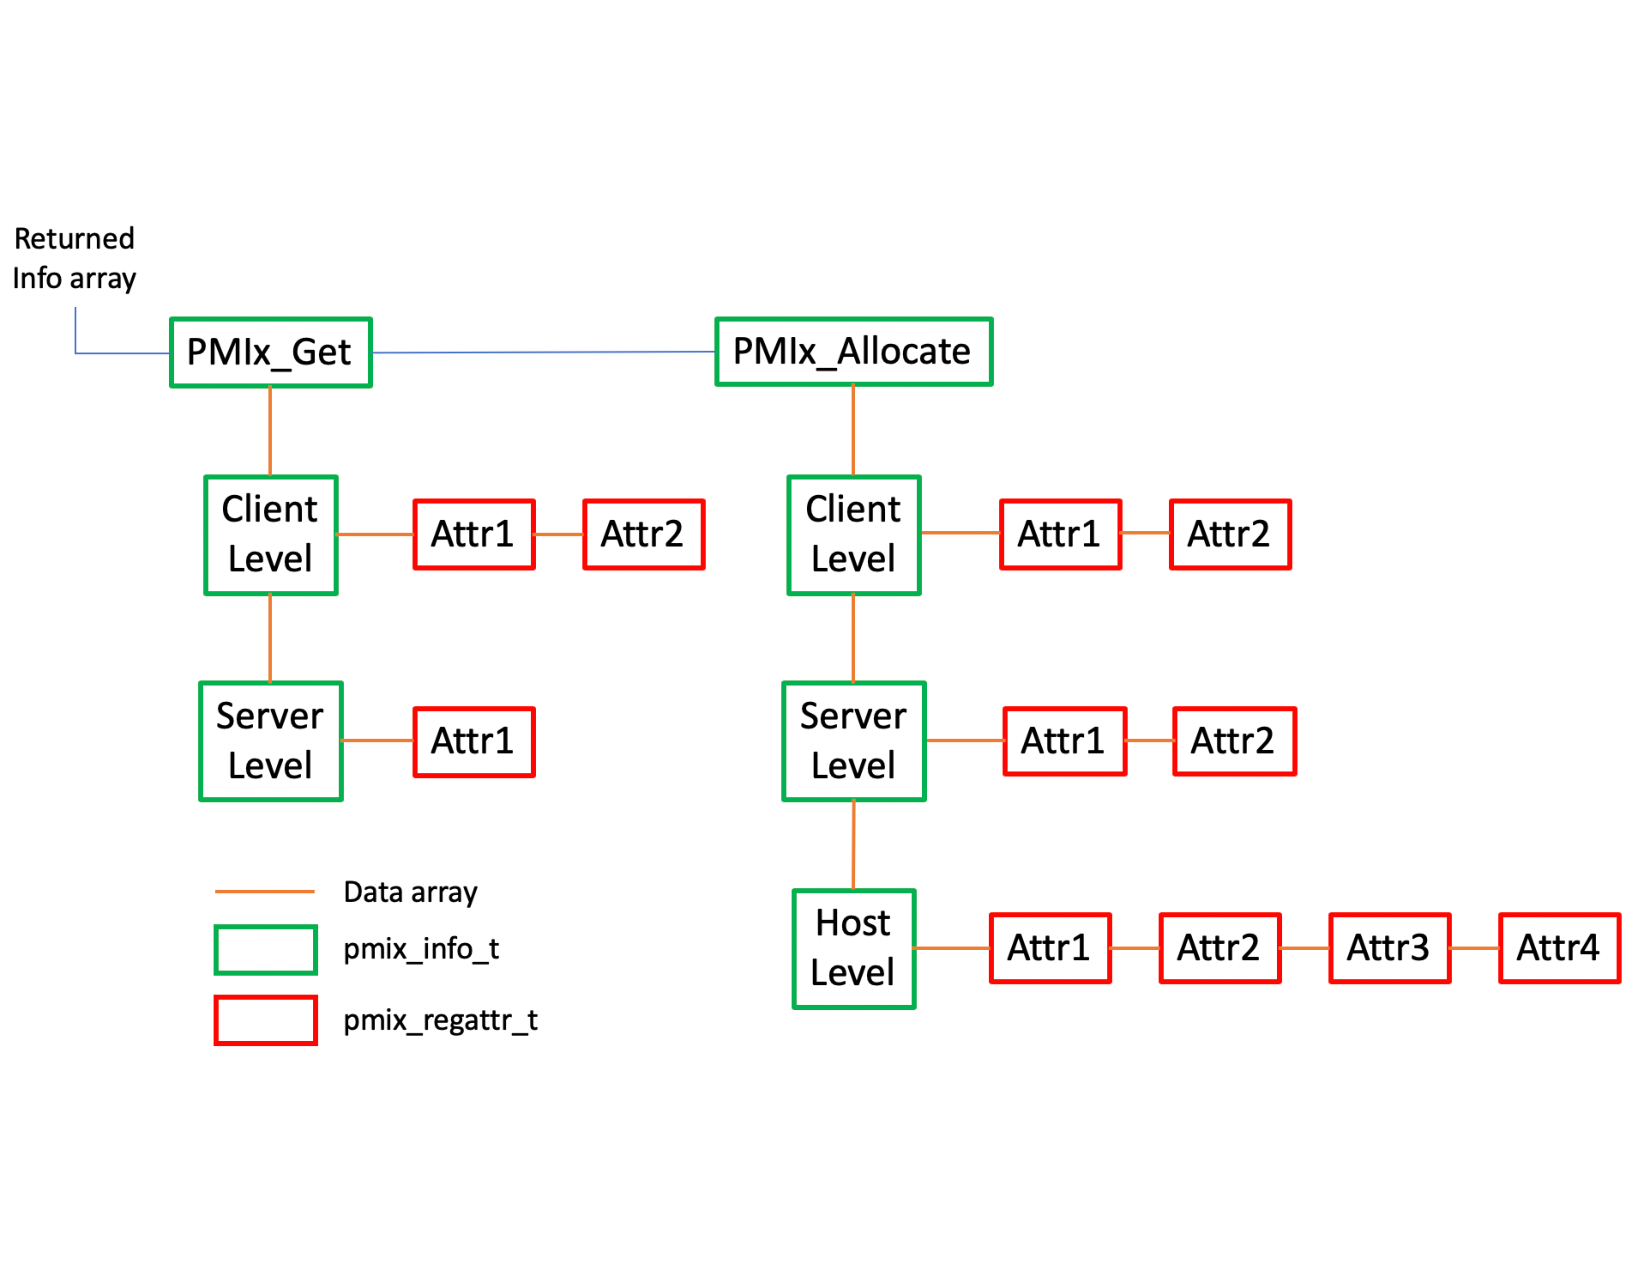
\includegraphics[clip,width=0.8\textwidth]{figs/attrquery.pdf}
  \end{center}
  \caption{Returned information hierarchy for attribute support request}
  \label{fig:attrquery}
\end{figure*}
\endgroup

The array of returned structures, and their child arrays, are subject to the return rules for the \refapi{PMIx_Query_info_nb} \ac{API}. For example, a request for supported attributes of the \refapi{PMIx_Get} function that includes the \refarg{host} level will return values for the \refarg{client} and \refarg{server} levels, plus an array element with a \refarg{key} of \refattr{PMIX_HOST_ATTRIBUTES} and a value type of \refconst{PMIX_UNDEF} indicating that no attributes are supported at that level.

%%%%%%%%%%%%%%%%%%%%%%%%%%%%%%%%%%%%%%%%%%%%%%%%%
